% ----------------------------- Design ---------------------------------------

\section{Design}

\subsection{Technical Environment}
% Mention minimum hardware configuration, software tools and package details.
\noindent
The technical environment for the project "Analyzing Social Media Posts for Mental Health Disorder Detection" comprises a combination of hardware, software, and tools that enable smooth data analysis, machine learning model training, and deployment. Below is a detailed overview of the minimum hardware configuration, software tools, and package details necessary to carry out this project effectively. \\

\noindent
\textbf{Minimum Hardware Configuration} \\
\noindent
Given the nature of the project, which involves processing textual data and training machine learning models, the hardware requirements are modest but significant enough to ensure optimal performance. The minimum configuration needed is:
\begin{itemize}
    \item \textbf{Processor} :
    \noindent
    Intel Core i5 (or equivalent) with a base clock speed of at least 2.5 GHz. A multi-core processor is preferred as it helps in parallel processing, which is essential during model training and data preprocessing steps.
    \item \textbf{RAM} :
    \noindent
    8 GB of RAM is recommended to handle the operations of data loading, cleaning, and transformation. Large datasets, like those used in this project, may require more memory to prevent memory overflow errors and reduce delays during processing. For larger datasets, 16 GB of RAM would be ideal.
    \item \textbf{Storage} :
    \noindent
    At least 256 GB of SSD storage is recommended. Faster storage access significantly impacts loading time for datasets and dependencies. SSD is preferred over traditional HDD because of its faster read/write speeds, which benefit large datasets like the Reddit-based social media posts used in this project.
    \item \textbf{Graphics Processing Unit (GPU)} :
    \noindent
    For basic machine learning tasks like Logistic Regression or SVM, a dedicated GPU is not necessary. However, if deep learning models or more complex neural networks were introduced later, a GPU like NVIDIA GTX 1060 with 4 GB VRAM or higher would be advantageous.
    \item \textbf{Operating System} :
    \noindent
    Windows 10 (64-bit) or higher, macOS 10.13 (High Sierra) or higher, or any stable Linux distribution (e.g., Ubuntu 18.04 or higher). The operating system should support all necessary machine learning libraries and be compatible with the tools required for the project.
\end{itemize} 

\noindent
\textbf{Software Tools and Packages} \\
\noindent
For the software stack, the project leverages a set of well-established tools, platforms, and programming libraries to ensure smooth execution from data preprocessing to model deployment:
\begin{itemize}
    \item \textbf{Python} :
    \noindent
    The primary programming language used for data processing, model training, and evaluation. Python is chosen due to its rich ecosystem of libraries and frameworks tailored for machine learning and data science.
    
    \item \textbf{Pandas} :
    \noindent
    A powerful library for data manipulation and analysis, essential for data preprocessing tasks, such as handling missing values and restructuring datasets.
    
    \item \textbf{scikit-learn} :
    \noindent
    A comprehensive machine learning library in Python used for implementing and comparing algorithms in classification, regression, and clustering, along with various model evaluation tools.
    
    \item \textbf{Streamlit} :
    \noindent
    An open-source Python framework that facilitates the deployment of machine learning models and interactive web applications.
    
    \item \textbf{Pyngrok} :
    \noindent
    A Python wrapper for ngrok, used to create secure tunnels to locally deployed applications, which is particularly useful for sharing Streamlit applications over the web.
    
    \item \textbf{Google Colab} :
    \noindent
    A cloud-based platform used for writing, executing, and sharing Python code, with access to GPU and TPU resources, beneficial for model training. It integrates seamlessly with libraries like TensorFlow and PyTorch.
    
    \item \textbf{PRAW (Python Reddit API Wrapper)} :
    \noindent
    A Python library that allows for easy interaction with the Reddit API to access, retrieve, and analyze Reddit data, such as posts, comments, and user information.

    \item \textbf{pytesseract} :
    \noindent
    A Python wrapper for Tesseract OCR, used to extract text from images. It's essential for converting image-based text data into a format suitable for processing.
    
    \item \textbf{Pillow} :
    \noindent
    A Python Imaging Library that adds support for image processing, which aids in handling image files for text recognition tasks with pytesseract.

    \item \textbf{joblib} :
    \noindent
    A library for efficient serialization and deserialization of Python objects, especially useful for saving and loading machine learning models during deployment.
    
    \item \textbf{protobuf} :
    \noindent
    A protocol buffer library by Google used for serializing structured data, helpful in efficient data exchange between applications.
    
    \item \textbf{deep-translator} :
    \noindent
    A library that facilitates easy translation across different languages, enabling multilingual processing of text data.
    
    \item \textbf{Requests} :
    \noindent
    A user-friendly library for making HTTP requests, used to retrieve data from APIs or web resources as part of data collection.
    
    \item \textbf{google-generativeai} :
    \noindent
    A Python client library for Google’s generative AI models, providing tools to integrate and utilize AI functionalities within the project.
    
\end{itemize}


\subsection{Hierarchy of Modules}
% Provide a diagram.
\begin{figure}[h!]  
    \centering
    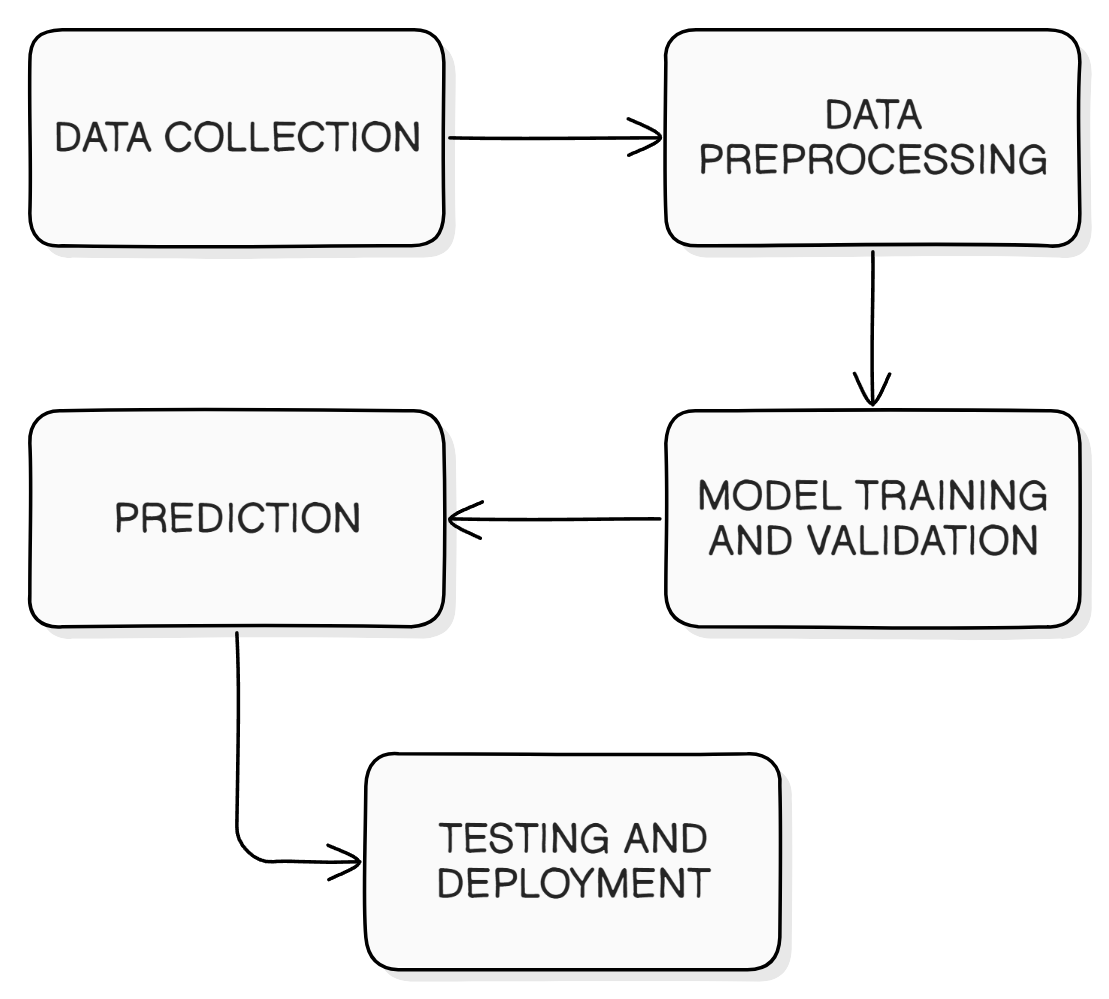
\includegraphics[width=0.6\textwidth]{Images/Project Modules.png}  
    \caption{Project Modules}
    \label{Project Modules}  % Label for referencing the figure
\end{figure}

\noindent
In this project, the system is structured into key modules to classify mental health issues based on text input effectively. The \textbf{Data Collection Module} gathers relevant text data, building a comprehensive dataset from sources like CSV files or platforms such as Reddit via PRAW. Next, the \textbf{Data Preprocessing Module} loads and cleans this data through tokenization, stop-word removal, and lemmatization, preparing it for analysis. Following this, the \textbf{Model Training and Validation Module} converts the text into numerical features using techniques like TF-IDF, Bag Of Words Model, splitting the data into training and validation sets to test various machine learning models, including Logistic Regression, Naive Bayes, SVM, Random Forest, XGboost, LSTM and Transformer. Next, the \textbf{Prediction Module} is for classification and displaying result. Finally, the \textbf{Testing and Deployment Module} allows real-time predictions by deploying the model on platforms like Streamlit Cloud, providing an accessible solution for practical applications.

\subsection{Detailed Design}
% Provide hierarchy of modules or overall system diagram. 
% \vspace{.1in}
\begin{figure}[h!]  
    \centering
    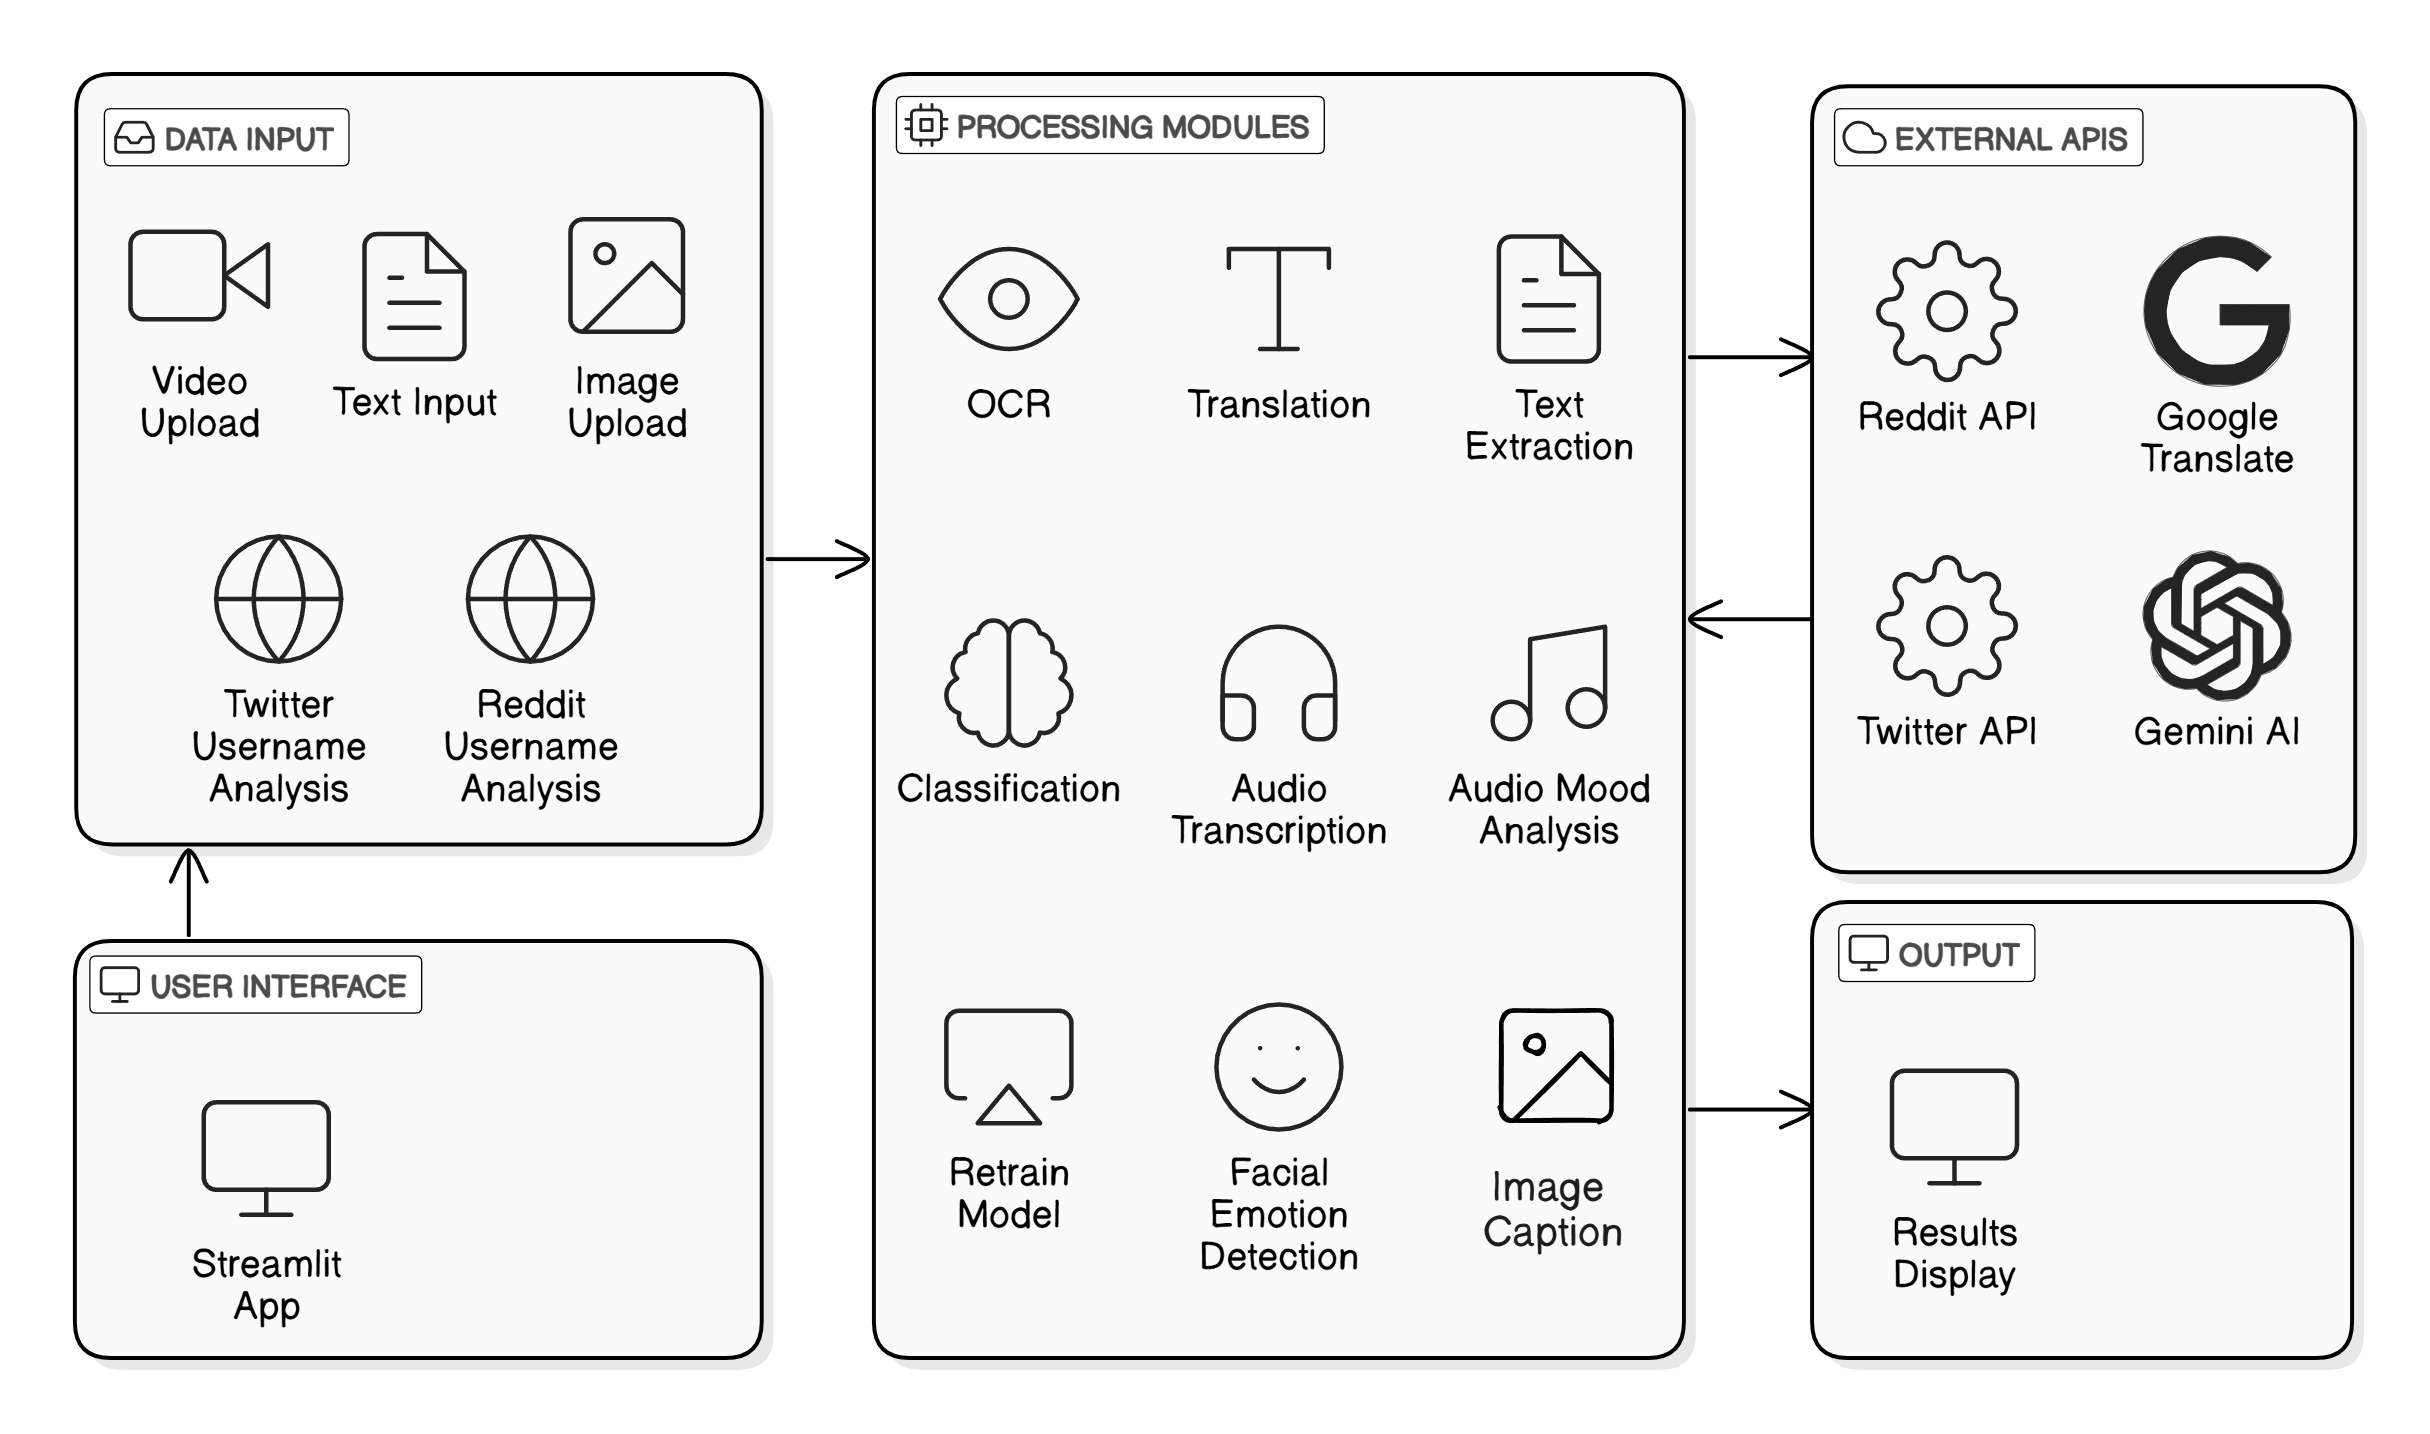
\includegraphics[width=1.0\textwidth]{Images/System Overview.png}  
    \caption{System Overview}
    \label{System Overview}  % Label for referencing the figure
\end{figure}


% \noindent
% For Detailed Design, use flowcharts, DFD, UML or ER diagrams as applicable. Titles of s7.2.1, 7.2.2 etc. should be with the name of respective design modules. Your focus should be on: “How the requirement will be implemented in the system?” Design Reference subsection numbers should be matching as stated in Requirement Matrix.
\vspace{.1in}

\subsubsection{Data Loading and Preprocessing}
\noindent
The Data Loading and Preprocessing Module is the foundation of the system, responsible for ingesting and preparing the text data for analysis. This module begins by loading the dataset from the mental\_health.csv file, which contains various mental health-related text entries. Once the data is loaded, a series of preprocessing steps are conducted to ensure the text is clean and ready for feature extraction. This includes tokenization, where the text is split into individual words or tokens, and lowercasing to maintain uniformity across the dataset. Additionally, stop-word removal is performed to eliminate common words that do not contribute to the meaning, such as "and," "the," and "is." Finally, lemmatization or stemming is applied to reduce words to their base or root forms.

\subsubsection{Feature Extraction}
\noindent
In the Feature Extraction Module, the preprocessed text data is transformed into a numerical format that machine learning algorithms can process. This module allows for the selection between two primary feature extraction methods: Term Frequency-Inverse Document Frequency and Bag Of Words Model.

\subsubsection{Model Training and Validation}
\noindent
The Model Training and Validation Module is critical to developing a robust classification system. In this module, the dataset is split into training and testing sets to evaluate the performance of the models accurately. Various classification algorithms are employed, including Logistic Regression, Naive Bayes, Support Vector Machines, Random Forest, XGboost, K-Nearest-Neighbours, LSTM and Transformer. Each model is trained on the training set, which involves adjusting the model parameters based on the input features and their corresponding labels. Following training, the models undergo validation to assess their performance. 

\subsubsection{Prediction}
\noindent
The Prediction Module is designed to provide real-time classification of new input text related to mental health issues. Upon receiving user input, this module initiates a preprocessing workflow that mirrors the steps applied during the training phase, including tokenization, lowercasing, stop-word removal, and lemmatization or stemming. Once the input text is preprocessed, it is fed into the trained classification models to generate predictions.

\subsubsection{Testing and Deployment}
\noindent
The module focuses on making the trained models accessible for real-time predictions. Once the models have been validated and selected based on their performance, this module prepares them for deployment on suitable platforms like Streamlit Cloud. This involves packaging the models and creating a user interface where users can input text and receive predictions. By providing a free and efficient deployment solution, this module enables users to access the mental health classification service easily. The deployment of the models ensures that the insights generated from the analysis can be utilized effectively in real-world applications.

\begin{figure}[h!]  
    \centering
    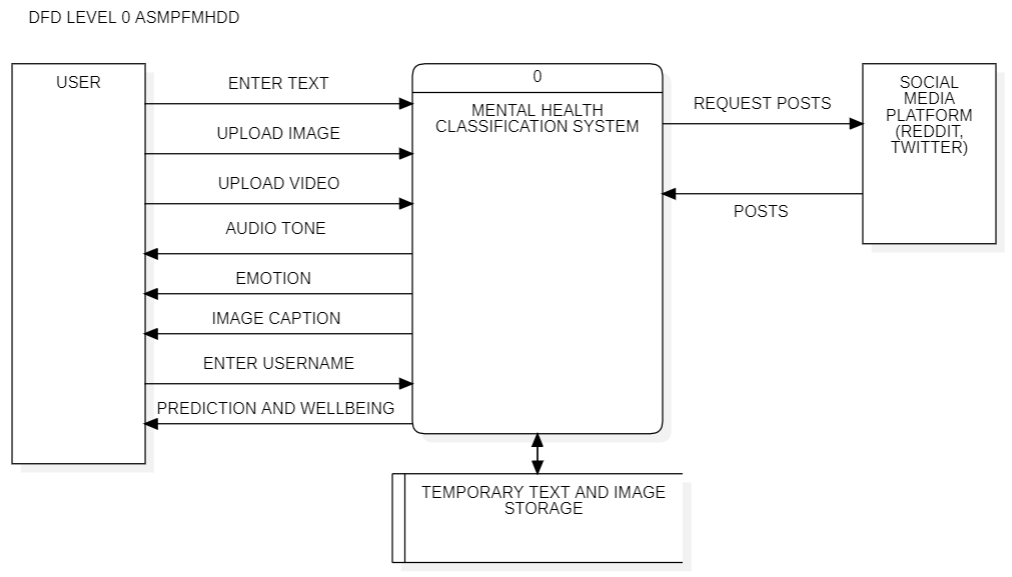
\includegraphics[width=0.7\textwidth]{Images/DFD L0.png}  
    \caption{DFD Level 0 of the System}
    \label{dfdl0123}  % Label for referencing the figure
\end{figure}

\pagebreak

\begin{figure}[h!]  
    \centering
    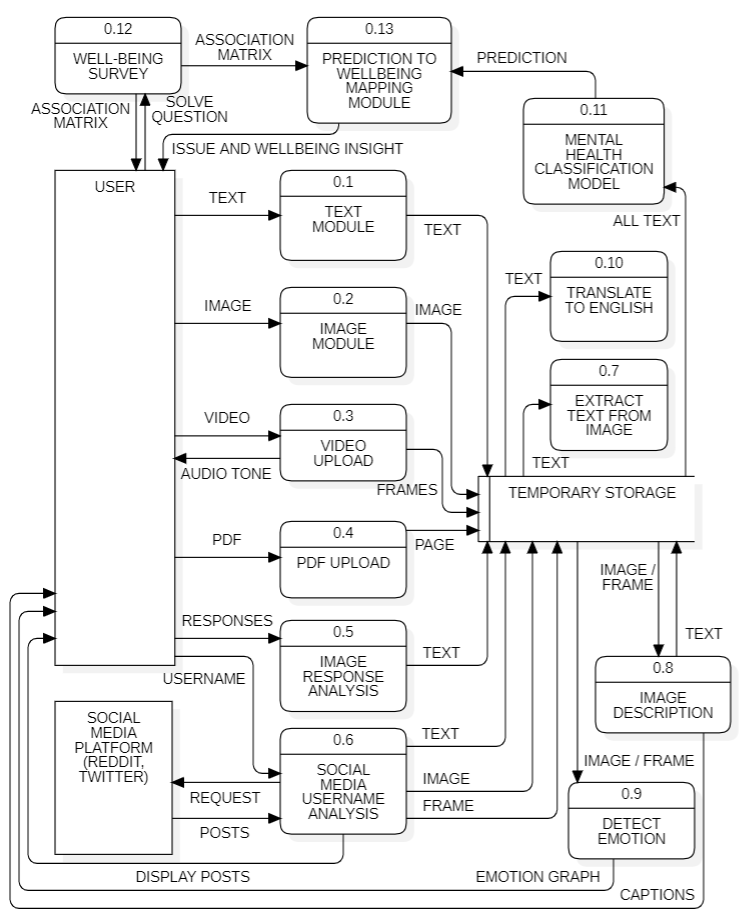
\includegraphics[width=0.65\textwidth]{Images/DFD L1.png}  
    \caption{DFD Level 1 of the System}
    \label{dfdl1234}  % Label for referencing the figure
\end{figure}

\pagebreak

\subsection{Emotion Detection Functionality}

\begin{figure}[h!]  
    \centering
    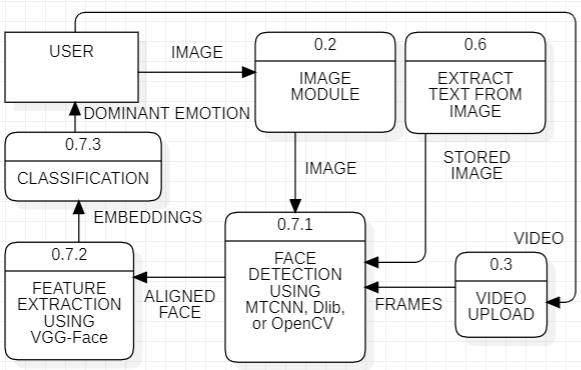
\includegraphics[width=0.7\textwidth]{Images/DFD L2 EMOTION.png}  
    \caption{DFD Level 2 of Emotion Detection Functionality}
    \label{dfdl14456}  % Label for referencing the figure
\end{figure}

\noindent
DeepFace analysis involves several steps to process and analyze facial features from an uploaded image or video frame. The process begins with the user uploading the input, which is passed to DeepFace’s pipeline. The first step is face detection, where models like MTCNN, Dlib, or OpenCV locate faces within the image. MTCNN (Multi-task Cascaded Convolutional Networks) detects faces using cascaded CNNs for high accuracy and alignment, while Dlib employs histogram-oriented gradients and machine learning techniques for robust detection. OpenCV, a widely-used computer vision library, uses Haar cascades or DNN-based approaches to detect faces. Once detected, the faces are cropped and aligned for consistency. Next is feature extraction, where pre-trained models like VGG-Face (a deep CNN trained specifically for face recognition) or Facenet (which uses triplet loss to generate highly discriminative face embeddings) convert the aligned face into numerical vectors called embeddings. These embeddings are compared using techniques like cosine similarity or Euclidean distance for tasks such as emotion detection(e.g., happiness, sadness), demographic analysis (e.g., age, gender), or face verification (matching two faces). Finally, the results, such as detected emotions or attributes, are displayed to the user, completing the analysis pipeline.


\subsection{Extract Text From Image}

\begin{figure}[h!]  
    \centering
    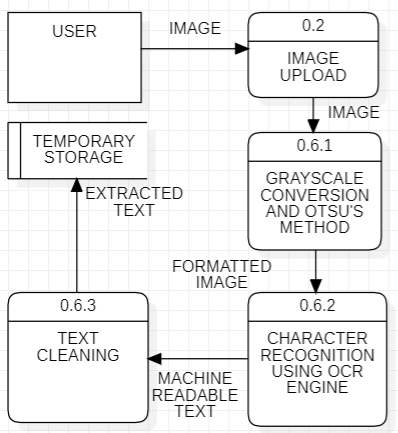
\includegraphics[width=0.5\textwidth]{Images/DFD L2 TEXT EXTRACT.png}  
    \caption{DFD Level 2 of Text Extraction from Image}
    \label{dfdl13456}  % Label for referencing the figure
\end{figure}

\noindent
The process of extracting text from an image using Tesseract-OCR begins with the user uploading an image containing text, such as a scanned document or a photo of a sign. This raw input undergoes preprocessing to enhance the image for OCR recognition. The first step in preprocessing is grayscale conversion, where the image’s RGB values are reduced to a single intensity value using a weighted formula. This simplifies the image by removing color information while retaining the text regions. Next, noise reduction is applied using techniques like Gaussian Blur or Median Blur, which smooth out artifacts while preserving the edges of text. After noise reduction, binarization is performed to convert the grayscale image into a binary format (black-and-white) using methods like Otsu’s thresholding. This step isolates the text from the background. Region detection follows, where text-heavy areas are identified using contour detection or connected component analysis, filtering out non-text regions based on properties like aspect ratio and alignment. Once preprocessing is complete, the image is passed to Tesseract for character recognition. This involves segmenting the image into text lines and individual characters, which are then processed by Tesseract’s LSTM-based neural network. The network evaluates sequences of characters in context, improving the accuracy of word recognition. Recognized characters are combined into machine-readable text, leveraging language models and dictionary lookups to maintain the natural flow and correct structure of the text. The output is a string of recognized text, but it may still require postprocessing for better accuracy and readability. Postprocessing begins with error correction, where the recognized text is compared against dictionaries or spell-checking algorithms to identify and fix errors caused by OCR misrecognition. Rule-based corrections are also applied, such as replacing common misinterpreted characters (e.g., \`0\` with \`O\` or \`l\` with \`1\`) depending on the context. After error correction, formatting is applied to structure the text into paragraphs, reconstruct line breaks, and retain alignments. This ensures that the extracted text is not only accurate but also well-organized for further use. Finally, the extracted text is either displayed to the user or saved to a file format such as \`.txt\` or \`.docx\`. This structured and cleaned output can then be utilized for various applications, from document analysis to content storage. The entire pipeline, from preprocessing to postprocessing, ensures a high-quality extraction process by combining image enhancement, deep learning-based recognition, and advanced text correction methods.


\subsection{Image Description}

\begin{figure}[h!]  
    \centering
    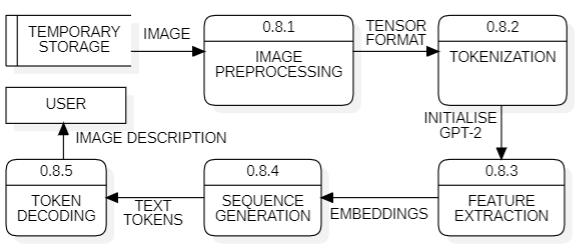
\includegraphics[width=0.7\textwidth]{Images/DFD L2 ID.png}  
    \caption{DFD Level 2 of Image Description}
    \label{dfdl122}  % Label for referencing the figure
\end{figure}

\noindent
The process of generating an image description using Python’s Transformers module and the ViT-GPT2 model begins with the user input, where the user uploads an image to be described. This image can be in any format (e.g., PNG, JPEG), and it is the raw data that will undergo a series of transformations before the description is generated. Once the image is received, it proceeds to the preprocessing stage. Preprocessing involves multiple steps: first, the image is resized to match the input dimensions required by the Vision Transformer (ViT) model, typically \(224 \times 224\) pixels. This ensures uniformity across all input data. The pixel values are then normalized to fall within a standard range (e.g., between 0 and 1), which improves the efficiency and stability of the model's computations. The image is subsequently transformed into a tensor format, which is the data structure required for processing by PyTorch or TensorFlow-based deep learning models. At this stage, the **GPT-2 tokenizer** is also initialized, preparing it to convert tokens into text during the sequence generation phase. Following preprocessing, the system moves to feature extraction, where the Vision Transformer (ViT) processes the image to extract meaningful features. ViT divides the image into smaller patches, typically \(16 \times 16\) pixels, and flattens each patch into a vector. These vectors are embedded using a linear projection layer, and positional embeddings are added to encode the spatial arrangement of the patches. The embedded patches are then passed through several transformer layers, where self-attention mechanisms analyze relationships between patches to capture both local and global image features. The final output of ViT is a high-dimensional embedding vector that represents the visual content of the image. This embedding vector is then passed to the GPT-2 decoder for the sequence generation phase. GPT-2 uses the image embeddings as input and applies its pre-trained language model to generate a sequence of text tokens. This is achieved through an iterative process where GPT-2 predicts the next token in the sequence based on the embeddings and previously generated tokens. The model continues this process until it reaches a stopping condition, such as an end-of-sequence (EOS) token. The generated tokens are numerical representations of words and phrases. Next comes the postprocessing stage, where the numerical tokens generated by GPT-2 are decoded back into human-readable text using the GPT-2 tokenizer. This step involves mapping the numerical tokens to their corresponding words in the vocabulary. The decoded text is then cleaned up for readability, ensuring proper grammar and structure. Any formatting issues are addressed during this stage to produce coherent and meaningful sentences. Finally, the system outputs the image description to the user. The description is a concise and accurate textual representation of the image content, such as “A group of people playing soccer on a field.” This description can be displayed on the application’s interface or saved to a file for further use. By leveraging the advanced capabilities of the Vision Transformer for feature extraction and GPT-2 for language modeling, this pipeline provides an efficient and accurate solution for automated image captioning.


\subsection{Translation to English}

\begin{figure}[h!]  
    \centering
    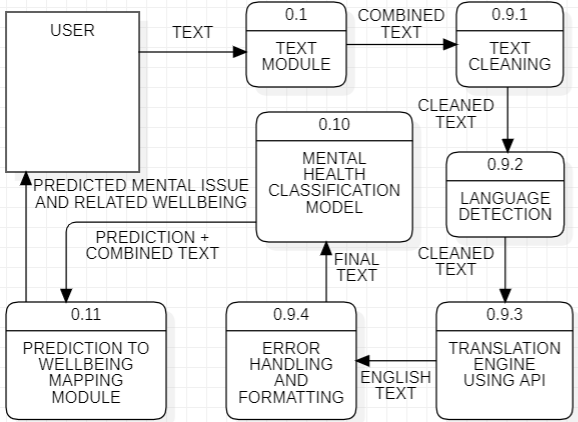
\includegraphics[width=0.7\textwidth]{Images/DFD L2 TE.png}  
    \caption{DFD Level 2 of Translation to English}
    \label{dfdl111}  % Label for referencing the figure
\end{figure}

\noindent
The process of translating text to English using DeepTranslator begins with the user providing input, either by typing text in a non-English language or uploading a file containing text. This input is handled by the system, which prepares it for translation. The text is first preprocessed to ensure optimal translation results. This involves cleaning the input by removing unwanted characters such as extra whitespace, punctuation errors, or HTML tags that could interfere with accurate translation. If the source language is not specified, a language detection step is performed. This step uses machine learning models trained on multilingual datasets to analyze patterns in the text, such as character distribution and word frequency, to determine the language. Models like Google’s Compact Language Detector employ statistical and supervised learning methods for this purpose. Once the text is prepared, it is passed to the DeepTranslator module, which interfaces with translation APIs like Google Translate or Microsoft Translator. These APIs rely on advanced neural machine translation (NMT) techniques to perform the translation. NMT models, which are based on deep learning, use sequence-to-sequence (seq2seq) architectures with encoder-decoder frameworks. The encoder processes the input text and converts it into a latent representation, a numerical vector capturing its meaning. This representation is then passed to the decoder, which generates the translated text in English. To ensure contextual accuracy, these models utilize attention mechanisms, which help focus on relevant parts of the input sentence during translation. Modern transformer-based architectures, like those used in Google Translate, enhance translation performance by enabling parallel processing of text and capturing long-range dependencies in sentences. After translation, the system postprocesses the output to ensure quality and readability. This includes validating the translated text for completeness, handling errors like untranslated phrases, and retrying failed requests if necessary. The output is formatted to resemble the original structure of the input, preserving elements like paragraphs, line breaks, and punctuation to maintain coherence. Finally, the translated text is displayed or saved, ensuring it is clean, accurate, and easy to understand. Throughout this process, concepts from natural language processing (NLP), deep learning, and robust error handling are integrated to provide reliable and efficient translations.


\subsection{Prediction to Wellbeing Mapping}

\begin{figure}[h!]  
    \centering
    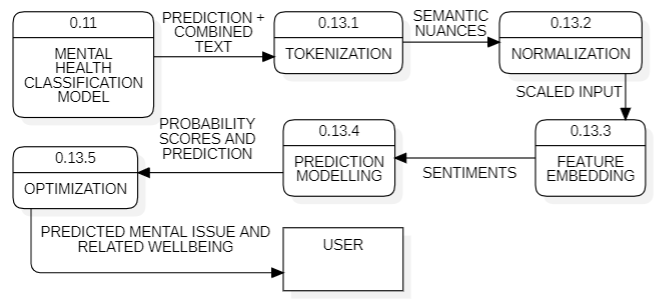
\includegraphics[width=0.7\textwidth]{Images/DFD L2 MW.png}  
    \caption{DFD Level 2 of Prediction to Wellbeing Mapping}
    \label{dfdl166}  % Label for referencing the figure
\end{figure}

\noindent
The process begins when the user provides input data for prediction, which could be in the form of text, behavioral data, or health metrics. For instance, a user might input their mood and health conditions, share behavioral patterns, or upload relevant data such as physical activity logs or medical records. This data serves as the foundation for predicting the user's mental health or overall wellbeing. Once the data is provided, the next step is preprocessing, which involves cleaning and transforming the raw input. During the data cleaning phase, any noise, missing values, or redundant information are identified and removed. This ensures the dataset is clean and ready for processing. Additionally, feature engineering is performed to extract meaningful attributes or characteristics from the raw data. For example, from behavioral data, features like activity frequency or sleep patterns may be derived. This allows the model to work with relevant information that enhances the prediction process. The third step involves embedding generation, where the core model, GEMINI 1.5 FLASH, processes the preprocessed input to generate embeddings. Embeddings are high-dimensional vectors that capture the semantic and contextual properties of the data. For example, when analyzing text input, GEMINI 1.5 FLASH uses its deep learning algorithms to understand the context and meaning of the user's words, transforming them into embeddings that encapsulate both the surface-level meaning and the deeper nuances of the data. This representation of the input data is essential for subsequent prediction tasks. In the prediction model phase, the generated embeddings are passed to machine learning models, which use these embeddings to predict a user's mental health status or behavioral outcomes. These models may utilize various algorithms, such as decision trees, support vector machines, or deep learning models, to make predictions. The system not only predicts the mental health condition but also maps these predictions to various wellbeing dimensions. These dimensions could include emotional wellbeing, such as happiness or stress; physical wellbeing, like energy levels or fatigue; and social wellbeing, including aspects like connectedness or isolation. By doing so, the system offers a comprehensive view of the user's overall wellbeing based on the predictions. Once predictions are made, postprocessing ensures the results are accurate and formatted properly. During the validation phase, the predictions are checked for any anomalies or inconsistencies, ensuring the output is reliable. This might involve techniques like consistency checks or outlier detection to verify that the predictions align with expected patterns. After validation, the results are formatted into a user-friendly structure. This might include organizing the wellbeing data into clear categories, such as emotional, physical, and social wellbeing, making it easy for the user to interpret. Finally, the system delivers the output, displaying or saving the prediction and associated wellbeing mapping. This output is presented in a way that helps the user understand the various aspects of their mental and physical health, giving them insights into their current state of wellbeing and providing actionable data for improvement.


\subsection{Audio Mood Analysis}

\begin{figure}[h!]  
    \centering
    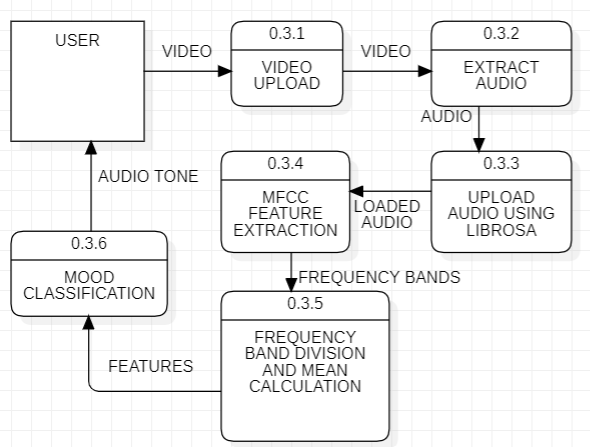
\includegraphics[width=0.7\textwidth]{Images/DFD L2 AM.png}  
    \caption{DFD Level 2 of Audio Mood Analysis}
    \label{dfdl671}  % Label for referencing the figure
\end{figure}

\noindent
The analyze\_audio\_mood function begins with the user providing a path to a video file as input. This is the starting point of the process where the user supplies the video from which the audio will be extracted. In the preprocessing stage, the video file is passed to the extract\_audio\_from\_video function. This function extracts the audio content from the video, separating it for further analysis. Once the audio is extracted, the next step involves loading the audio file into memory using the librosa library, which prepares the audio data for feature extraction. The core of the audio processing happens during the MFCC (Mel-frequency cepstral coefficients) feature extraction. The librosa.feature.mfcc method is used to compute the MFCCs of the audio. These MFCCs represent different frequency bands of the audio signal and are crucial for analyzing the characteristics of the audio that correspond to various emotional tones. By capturing frequency patterns, MFCCs provide a robust feature set for mood classification. After the MFCCs are extracted, the next step is feature segmentation. The MFCC array is divided into four distinct frequency bands: low frequencies (MFCCs 0, 1, and 2), mid-low frequencies (MFCCs 3 and 4), mid-high frequencies (MFCCs 5, 6, and 7), and high frequencies (MFCCs 8, 9, 10, 11, and 12). For each of these frequency bands, the scalar mean of the MFCC values is computed. This scalar mean represents the overall intensity of the audio in each frequency range, simplifying the data for classification purposes. Finally, the mood classification process takes place. The scalar means for each of the frequency bands are compared to determine the dominant mood of the audio. Based on these comparisons, the function classifies the audio as normal, neutral, melancholic, calm, anxious, or happy, depending on which frequency bands exhibit the strongest characteristics. This mood classification is then returned as the result of the analysis. The audio classification can be further improved using Gemini API thorugh a detailed prompt and display the tone, mood and summary for the respective audio.

\vspace{1em}

\noindent
The various processes and technologies discussed throughout this conversation can play a pivotal role in enhancing the classification and prediction of mental health disorders. The use of machine learning (ML) and deep learning (DL) models enables the system to process and analyze large volumes of data, such as text, behavioral patterns, health metrics, and even multimedia inputs (e.g., images, audio, and video). By leveraging the DeepFace module for facial emotion recognition, the system can identify emotional cues from visual data, helping to assess a user’s emotional state. This is complemented by text analysis models, such as those built with Logistic Regression, Naive Bayes, SVM, Transformer, XGboost and LSTM architectures, which are capable of classifying mental health issues from user-provided text, such as social media posts, personal narratives, or other forms of written communication. By incorporating audio mood analysis through techniques such as MFCC for audio emotion detection and facial expression recognition for video inputs, the system further refines its ability to assess emotional and mental states. These audio and visual analyses provide additional layers of understanding that text alone might not fully capture. In conjunction with these features, streaming data from social media platforms like Reddit or Twitter allows for the monitoring of a user’s public posts, providing real-time insights into their mental health as they interact with others online. 



% \noindent
% Create separate sections for separate modules of design as in Requirement Matrix. Ensure to provide Design Diagrams \textit{(e.g. System overview / DFDs / ERDs etc.; cross-reference to be drawn from Chapter 6), Decision matrix (for algorithm recommendation etc.) }




% \subsubsection{Name of Design Module 1 \label{sec:design_mod1}}
% \subsubsection{Name of Design Module 2 \label{sec:design_mod2}}
% \subsubsection{Name of Design Module 3 etc \label{sec:design_mod3}}


% Refer APPENDIX A  – Prototypes \ref{sec:proto} for prototype details.


% ------------------------------ Design Ends ---------------------------------

